\documentclass[lang=en,a4paper,11pt,openany,twoside]{elegantbook}

\let\arrowvert\relax
%\usepackage{unicode-math}

\let\arrowvert\relax


\usepackage{xeCJK}
\usepackage{amsmath} % 建议
\usepackage{amssymb} % 可选,提供更多符号

\usepackage{ctex}
\let\openbox\relax

\usepackage{tikz}
\usetikzlibrary{decorations.pathreplacing,arrows.meta}

%调整页边距
\usepackage{geometry}
\geometry{top=2cm, bottom=2.25cm, outer=2cm, inner=2.5cm}


\usepackage{setspace}
\setstretch{1.3}

%设定行间距
\usepackage{calc}
\setlength{\lineskip}{\baselineskip-\ccwd}
\setlength{\lineskiplimit}{2.5pt}



%浮动图片
\usepackage{wrapfig}
%图标表格注记
\usepackage{caption}
%圆圈数字
\usepackage{pifont}
%表格换行
\usepackage{makecell}
%表格颜色
\usepackage[table]{xcolor}
\colorlet{rowcolcolor}{structurecolor!25!white}

%行间距加大
\newcommand{\wideline}{\setlength{\lineskip}{\baselineskip-\ccwd}\setlength{\lineskiplimit}{2.5pt}}
%蓝色加粗
\definecolor{titleblue}{HTML}{3498DB}
\newcommand{\bluebf}[1]{\textcolor{structurecolor}{\textbf{#1}}}


%向量
\usepackage[f]{esvect}

\renewcommand{\vector}[1]{\vv{#1}}
%平面
\newcommand{\plane}{\text{平面}\ }
%平行且等于
\newcommand{\paraleq}{%
    \mathrel{\text{%
        \tikz[baseline]
        \draw (.1em,0ex) -- (.9em,0ex)
        (.1em,-.425ex) -- (.9em,-.425ex)
        (.350em,.1ex) -- (.650em,1.5ex)
        (.550em,.1ex) -- (.850em,1.5ex);}}}

\newcommand{\mb}{\mathbb}
\newcommand{\z}{\text}
\renewcommand{\a}{\alpha}
\renewcommand{\b}{\beta}
\renewcommand{\d}{\mathrm{d}}
\newcommand{\D}{\Delta}
\renewcommand{\l}{\lambda}
\newcommand{\m}{\mu}
\newcommand{\fl}{\fillin}
\newcommand{\pr}{\paren}
\newcommand{\p}{\uppi}
\renewcommand{\th}{\theta}
\newcommand{\lam}{\lambda}
\newcommand{\rttri}{\mathrm{Rt}\triangle}
\newcommand{\npar}{\par\noindent}
\DeclareSymbolFont{ugmL}{OMX}{mdugm}{m}{n}
\DeclareMathAccent{\wideparen}{\mathord}{ugmL}{"F3}
\newcommand{\sigmaalg}{\sigma-\text{代数}}
\newcommand{\setjot}[1][0]{\setlength{\jot}{#1 pt}}


%填空题下划线
\newcommand{\fillin}[1][3.5]{%
  \nolinebreak % 不在此处断行
  \hspace{0.2em}%
  \rule[-0.5ex]{#1em}{0.5pt}% 轻微下沉模拟“下划线”效果
  \hspace{0.05em}
}

%调整环境内图片环绕
\usepackage{mwe}
\newcommand{\wrapfix}[1][-1]{\begin{wrapfigure}{r}{0.001\textwidth}%
    \vspace{#1 em}%
    \includegraphics[width=0.001\textwidth]{example-image}%
    \end{wrapfigure}}


%分式使用行间版
\everymath{\displaystyle}


\usepackage{myenvironment}


%elegantbook部分修改
\usepackage{elegantfix}

%强制右页开始
\makeatletter
\newcommand{\ForceRightPage}{%
  \clearpage
  \ifodd\value{page}\relax
    % 已经是奇数页,什么也不做
  \else
    \hbox{}\thispagestyle{empty}\newpage
  \fi
}
\makeatother

\renewcommand{\figurename}{Figure}
\renewcommand{\tablename}{Table}
\renewcommand{\contentsname}{Contents}

\raggedbottom


\begin{document}


\title{Notes for Differential Geometry}
\date{}
\maketitle
\setcounter{page}{1}

\frontmatter
\pagenumbering{roman}     % 目录等用罗马数字
\clearpage
\tableofcontents
\clearpage

\ForceRightPage
\mainmatter

\chapter{Curves}

\section{Parameterized Curves}

\begin{definition}{Parameterized curve}
    A parameterized curve is a smooth map $c:I\to\mathbb{R}(n=2,3)$,where $I$ is an interval,usually $[a,b]$ or $(0,1)$.
\end{definition}



\begin{definition}{Curve}
    A curve is the image $c(I)$ of a parameterized curve $c$.
\end{definition}

\begin{definition}{Velocity}
    The velocity of a parameterized curve $c(t)$ is $\dot{c}(t)=\frac{\d c}{\d t}(t)=\lim_{h\to 0}{\frac{c(t+h)-c(t)}{h}}\in\mathbb{R}^n$.\par


    If  $c(t)=\begin{pmatrix}
        c_1(t) \\ c_2(t) \\ \vdots \\ c_n(t)
    \end{pmatrix}$, then $\dot{c}(t)=\begin{pmatrix}
        \dot{c_1}(t) \\ \dot{c_2}(t) \\ \vdots \\\dot{c_n}(t)
    \end{pmatrix}$.
\end{definition}

\begin{definition}{Acceleration}
    The acceleration of a parameterized curve $c(t)$ is $\ddot{c}(t)=\frac{\d\dot{c}}{\d t}(t)=\frac{\d^2c}{\d t^2}(t)\in\mathbb{R}^n$.\par
    If  $c(t)=\begin{pmatrix}
        c_1(t) \\ c_2(t) \\ \vdots \\ c_n(t)
    \end{pmatrix}$, then $\ddot{c}(t)=\begin{pmatrix}
        \ddot{c_1}(t) \\ \ddot{c_2}(t) \\ \vdots \\\ddot{c_n}(t)
    \end{pmatrix}$.
\end{definition}

\begin{instance}
    The map $c(t)=\begin{pmatrix}
        \cos t \\ \sin t
    \end{pmatrix},\;t\in[0,2\pi]$ is a parametrization of the unit circle.\par
    And its velocity and acceleration is  $\dot{c}(t)=\begin{pmatrix}
        -\sin t \\ \cos t
    \end{pmatrix}$,$\ddot{c}(t)=-\begin{pmatrix}
        \cos t \\ \sin t
    \end{pmatrix}$.
\end{instance}

Now, I can give an example to show that whether a curve is smooth depends on its parametrization. Even though a curve is cusp,it can be smooth.\par

\begin{instance}
    \begin{figure}[h]
        \centering
        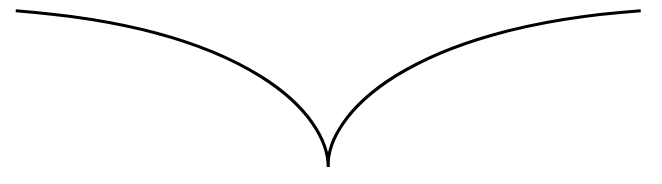
\includegraphics[width=0.4\textwidth]{fig/1.2.png}
        \captionof{figure}{}
    \end{figure}\par
    If we choose $c_1(t)=\begin{pmatrix}
        t \\ \sqrt{t}
    \end{pmatrix}$, the curve is not smooth because it is not derivable at $(0,0)$.\par
    When the parametrization is $c_2(s)=\begin{pmatrix}
        s^3 \\ s^2
    \end{pmatrix}$, it is a smooth one and its velocity is $\dot{c_2}(s)=\begin{pmatrix}
        3s^2 \\ 2s
    \end{pmatrix}$.
\end{instance}

\begin{definition}{Regularity}
    A parameterized curve is called regular if $\dot{c}(t)\neq 0\;\forall t\in I$.
\end{definition}

To calculate the length of a curve,we need the concept of inner product and norm.

\begin{definition}{Inner product and Norm}
    Inner product on $\mathbb{R}^n$ is $x\cdot y = \langle x,y \rangle=\sum_{i=1}^n{x_iy_i}$.\par
    Norm on $\mathbb{R}^n$ is $\|x\|=\sqrt{x\cdot x}=\sqrt{\sum_{i=1}^n{x_1\cdot x_i}}$.
\end{definition}

\begin{figure}[h]
    \centering
    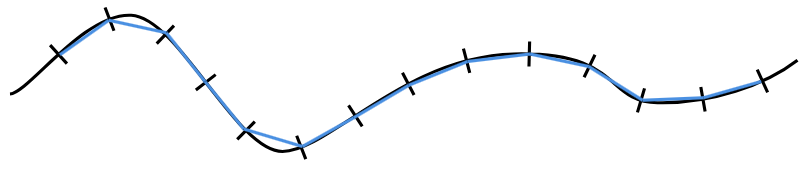
\includegraphics[width=0.6\textwidth]{fig/1.3.png}
    \captionof{figure}{}
\end{figure}

\begin{definition}{Length}
    A length of a parameterized curve $c(t)$ is $L(c) = \int_a^b{\|\dot{c}(t)\|}\,\d t$.
\end{definition}

\begin{instance}
    A unit circle has length $L(c)=\int_0^{2\pi}{\sqrt{\sin^2t+\cos^2t}}\,\d t=2\pi$.
\end{instance}

\begin{definition}{Diffeomorphism}
    If $\varphi:I_1\to I_2$ is a diffeomorphism
\end{definition}



\section{Parameterized curves}

There are two ways to view a curve. Imagine you register for a mountain bike race. The race track, as marked by the organizers, exists independently of you and is described by a certain set of points in space. This one-dimensional object is what we call a curve. However, as a participant in the race, you experience the curve differently: you move along it, and your position can be recorded at different times. This function, which maps time to your position in space, is what we refer to as a parameterized curve.

\begin{definition}{Parameterized curve}
    A parameterized curve is a smooth map \(c : I \rightarrow  {\mathbb{R}}^{n}\left( {n = 2,3}\right)\) , where \(I\) is an interval, usually \(\left\lbrack  {a,b}\right\rbrack\) or $(0,1)$.
\end{definition}

\begin{figure}[h]
    \centering
    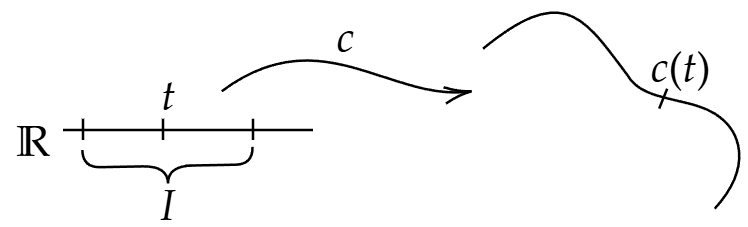
\includegraphics[width=0.5\textwidth]{fig/1.1.png}
    \captionof{figure}{}
\end{figure}

\begin{definition}{Curve}
    A curve is the image of a parameterized curve, i.e., the set \(\{ c\left( t\right)  : t \in  I\}\) .
\end{definition}


Note that the parameter \(t\) does not necessarily represent time; it can be any parameter that varies along the curve. For example, in the case of the bike race, \(t\) could represent the distance traveled along the track instead of the time elapsed. Nonetheless, it is often convenient to think of \(t\) as time, as it provides an intuitive way to understand the motion along the curve. In this spirit, we refer to \(\dot{c}\left( t\right)  = \frac{\mathrm{d}c}{\mathrm{\;d}t}\) as the velocity vector and \(\ddot{c}\left( t\right)  = \frac{\mathrm{d}\dot{c}}{\mathrm{\;d}t}\) as the acceleration vector.

There are many different parameterizations for the same curve. For example, different riders may travel at different speeds, leading to different parameterizations of the same physical curve. So we need a way to pass from one parameterization to another.

\begin{definition}{Diffeomorphism}
    A smooth map \(\varphi  : {I}_{2} \rightarrow  {I}_{1}\) is called a diffeomorphism if \(\varphi\) is bijective (one-to-one and onto) and its inverse \({\varphi }^{-1}\) is also smooth.
\end{definition}

\begin{definition}{Reparameterization}
    If \(\varphi  : {I}_{2} \rightarrow  {I}_{1}\) is a diffeomorphism with \({}^{a}{\varphi }^{\prime }\left( t\right)  > 0\) and \({c}_{1} : {I}_{1} \rightarrow  {\mathbb{R}}^{n}\) is a parameterized curve, then \({c}_{2}\left( t\right)  = {c}_{1}\left( {\varphi \left( t\right) }\right)  : {I}_{2} \rightarrow  {\mathbb{R}}^{n}\) is also a parameterized curve, called the reparameterization of \({c}_{1}\) by \(\varphi\) .

\({}^{a}\) A diffeomorphism \(\varphi\) always has either \({\varphi }^{\prime }\left( t\right)  > 0\) or \({\varphi }^{\prime }\left( t\right)  < 0\) for all \(t\) . The latter case would correspond to reversing the direction of the curve.
\end{definition}




We will often introduce a certain property of the curve using a parameterization, and then show that this property does not depend on the choice of parameterization. For example, the length of a curve is a property that should be independent of how we parameterize it - all riders should better agree on the length of the track, regardless of their speed.



Definition 4 (Length of a curve)

\begin{definition}{Length of a curve}
    The length of a parameterized curve \(c : I \rightarrow  {\mathbb{R}}^{n}\) is defined as

\[
L\left( c\right)  \mathrel{\text{ := }} {\int }_{a}^{b}\parallel \dot{c}\left( t\right) \parallel \mathrm{d}t \tag{1.1}
\]

where \(I = \left\lbrack  {a,b}\right\rbrack\) or(a, b).
\end{definition}

\begin{lemma}{}
    If \({c}_{2}\) is a reparameterization of \({c}_{1}\) , then the length of \({c}_{1}\) and \({c}_{2}\) are the same.
\end{lemma}

\begin{proof}
Since \({c}_{2}\left( t\right)  = {c}_{1}\left( {\varphi \left( t\right) }\right)\) for some diffeomorphism \(\varphi  : {I}_{2} \rightarrow  {I}_{1}\) , we have by the chain rule

\[
{\left. \frac{\mathrm{d}}{\mathrm{d}t}\right| }_{t}{c}_{2} = {\left. {\varphi }^{\prime }\left( t\right) \frac{\mathrm{d}}{\mathrm{d}s}\right| }_{\varphi \left( t\right) }{c}_{1}.
\]

Assume, without loss of generality, that \({I}_{1} = \left\lbrack  {{a}_{1},{b}_{1}}\right\rbrack\) and \({I}_{2} = \left\lbrack  {{a}_{2},{b}_{2}}\right\rbrack\) with \(\varphi \left( {a}_{2}\right)  = {a}_{1}\) and \(\varphi \left( {b}_{2}\right)  = {b}_{1}\) . Thus,

\[
L\left( {c}_{2}\right)  = {\int }_{{a}_{2}}^{{b}_{2}}\begin{Vmatrix}{{\left. \frac{\mathrm{d}}{\mathrm{d}t}\right| }_{t}{c}_{2}}\end{Vmatrix}\mathrm{d}t
\]

\[
= {\int }_{{a}_{2}}^{{b}_{2}}\left| {{\varphi }^{\prime }\left( t\right) }\right|  \cdot  \begin{Vmatrix}{{\left. \frac{\mathrm{d}}{\mathrm{d}s}\right| }_{\varphi \left( t\right) }{c}_{1}}\end{Vmatrix}\mathrm{d}t
\]

\[
s = \underline{\underline{\varphi }}\left( t\right) {\int }_{{a}_{1}}^{{b}_{1}}{\begin{Vmatrix}{\left. \frac{\mathrm{d}}{\mathrm{d}s}\right| }_{s}{c}_{1}\end{Vmatrix}}_{a}{ds}
\]

\[
= L\left( {c}_{1}\right) ,
\]
\end{proof}


where we used the reparameterization theorem for integrals in the third step.

The proof exhibits a general strategy that we will use often in this course: when we want to investigate a certain property of a curve or surface, we will use a parameterization to boil it down to a problem in calculus that we know how to solve. Here, we just used the chain rule and the reparameterization theorem for integrals.

At this point, a word of caution is in order. In the definition of a curve, we required the parameterization to be smooth (i.e, all derivatives exist and are continuous). However, this does not imply that the curve itself is smooth in a geometric sense. For example, the parameterization \(c\left( t\right)  = \left( {{t}^{3},{t}^{2}}\right)\) is smooth, but the curve it describes has a cusp at the origin.


Figure 1. Plot of the smooth curve \(c\left( t\right)  = \left( {{t}^{3},{t}^{2}}\right)\) showing a cusp at the origin.

To avoid such singularities, we introduce the following definition.


\begin{definition}{Regular curve}
    A parameterized curve \(c\) is called regular if \(\dot{c}\left( t\right)  \neq  0\) for all \(t \in  I\) . Such a curve, in particular, has no cusps or corners.
\end{definition}

The regularity condition ensures that the curve has a well-defined, non-zero tangent vector at every point, which is crucial for many applications in differential geometry. We will almost always assume that the curves we work with are regular. The following result shows that every regular curve can be reparameterized to have unit speed, which is often a convenient choice.

\begin{proposition}{}
    For every regular curve \(c : I \rightarrow  {\mathbb{R}}^{n}\) , there exists a diffeomorphism \(\varphi  : I \rightarrow  I\) such that \(\widetilde{c}\left( s\right)  = c\left( {\varphi \left( s\right) }\right)\) has unit-speed, i.e., \(\parallel \dot{\widetilde{c}}\left( s\right) \parallel  = 1\) for all \(s \in  I\) .
\end{proposition}



A curve \(c\left( t\right)\) with unit-speed is also called an \bluebf{arc-length parameterization} of the curve, since the parameter \(t\) directly measures the length along the curve from some starting point. Indeed, if we let \(l\left( t\right)  = {\int }_{{t}_{0}}^{t}\parallel \dot{c}\left( \tau \right) \parallel \mathrm{d}\tau\) be the length of the arc from a given point \(c\left( {t}_{0}\right)\) to \(c\left( t\right)\) , then for a unit-speed curve, we have \(l\left( t\right)  = t - {t}_{0}\) .

For a unit-speed curve, the velocity vector \(\dot{c}\left( t\right)\) has unit length by definition. We can use the acceleration to find a second vector \(N\left( t\right)\) that is perpendicular to \(\dot{c}\left( t\right)\) and also has unit length.



Theorem 1 (Moving frame)

\begin{theorem}{Moving frame}
    Let \(c : I \rightarrow  {\mathbb{R}}^{n}\) be a unit-speed curve with \(\ddot{c}\left( t\right)  \neq  0\) for all \(t\) , then
    \[
    T\left( t\right)  \mathrel{\text{ := }} \dot{c}\left( t\right) ,\;N\left( t\right)  \mathrel{\text{ := }} \frac{\ddot{c}\left( t\right) }{\parallel \ddot{c}\left( t\right) \parallel } \tag{1.2}
    \]
    have unit length and are perpendicular to each other, i.e., they form a pair of orthonormal vectors.
\end{theorem}

If the curve lies in \({\mathbb{R}}^{2}\) , then we get two orthonormal vectors \(T\left( t\right)\) and \(N\left( t\right)\) that span \({\mathbb{R}}^{2}\) , i.e., an orthonormal basis of \({\mathbb{R}}^{2}\) that moves along the curve. This is called a moving or Frenet-Serret frame along the curve.


\begin{definition}{Curvature}
    The curvature of a unit-speed curve \(c : I \rightarrow  {\mathbb{R}}^{n}\) is defined as \(\kappa \left( t\right)  = \parallel \ddot{c}\left( t\right) \parallel\) .
\end{definition}


What is the curvature of a general regular curve \(c : I \rightarrow  {\mathbb{R}}^{n}\) ? The natural definition is to first reparameterize \(c\) to a unit-speed curve \(\widetilde{c}\) by a suitable reparameterization \(\varphi\) and then define the curvature of \(c\) as the curvature of \(\widetilde{c}\) . One has to be a bit careful here to measure the curvature at the same point on the curve: If \(c\left( t\right)\) is a point on the curve, then \(\widetilde{c}\left( s\right)  = c\left( {\varphi \left( s\right) }\right)\) is the same point if \(s = {\varphi }^{-1}\left( t\right)\) . Accordingly, we define the curvature \(\kappa \left( t\right)\) of \(c\) at \(t \in  I\) as the curvature \(\widetilde{\kappa }\left( s\right)\) of \(\widetilde{c}\) at \(s = {\varphi }^{-1}\left( t\right)\) , i.e.,

\[
\kappa \left( t\right)  = \widetilde{\kappa }\left( {{\varphi }^{-1}\left( t\right) }\right) . \tag{1.3}
\]

\begin{lemma}{}
    If \(c : I \rightarrow  {\mathbb{R}}^{n}\) is a regular curve, then its curvature is given by
    \[
    \kappa \left( t\right)  = \frac{1}{v{\left( t\right) }^{2}}\sqrt{\parallel \ddot{c}\left( t\right) {\parallel }^{2} - \dot{v}{\left( t\right) }^{2}} = \frac{\sqrt{v{\left( t\right) }^{2}\parallel \ddot{c}\left( t\right) {\parallel }^{2} - {\left( \dot{c}\left( t\right)  \cdot  \ddot{c}\left( t\right) \right) }^{2}}}{v{\left( t\right) }^{3}}, \tag{1.4}
    \]
    where \(v\left( t\right)  = \parallel \dot{c}\left( t\right) \parallel\) is the speed of \(c\) at time \(t\) .
\end{lemma}


\section{Paddle on the moon}




\end{document}